% ============================================================================
%  Group 22 - Machine Learning, NOVA IMS
%  Handout: overall structure and rationale of the pipeline
%
%  OUTPUT NAME REQUIRED BY THE COURSE:  Group_22_handout_text.pdf
%  In Overleaf: Menu -> Settings -> "Default output name" -> Group_22_handout_text
%  Compiler: pdfLaTeX (it also compiles under XeTeX, which is what the local build uses).
%
%  LAYOUT: page 1 is the cover, pages 2 and 3 hold the report.
%
%  UPLOAD THESE TWO FILES INTO A "figures" FOLDER IN THE OVERLEAF PROJECT
%  (they are charts the notebooks draw, unchanged):
%      figures/nb04_model_comparison.png
%      figures/nb04_assessment.png
%
%  IF THE LAST PAGE SPILLS, shorten Annex C first, then the figure captions.
% ============================================================================
\documentclass[11pt,a4paper]{article}

\usepackage[T1]{fontenc}
\usepackage{lmodern}
\usepackage[margin=1.95cm,top=1.7cm,bottom=1.45cm]{geometry}
\usepackage{graphicx, booktabs, tabularx, xcolor, microtype}
\usepackage{tikz}
\usetikzlibrary{positioning, arrows.meta}
\usepackage{titlesec}

\titleformat{\section}{\normalfont\bfseries\large}{\thesection.}{0.6em}{}
\titlespacing*{\section}{0pt}{5pt}{2pt}

% One spacing rule for the whole document: a period is just a period, paragraphs are
% separated by a gap rather than by a first-line indent, and every bold lead-in is
% followed by exactly one space. Without \frenchspacing TeX stretches the space after
% the full stop in "Preprocessing." wide, which is what read as a stray tab.
\frenchspacing
\setlength{\parindent}{0pt}
\setlength{\parskip}{3pt plus 1pt minus 1pt}

\newcommand{\lead}[1]{\textbf{#1.}\space}
\newcommand{\anx}[1]{\textbf{#1.}\space}
\renewcommand{\arraystretch}{1.1}
\newcolumntype{R}{>{\raggedright\arraybackslash}X}
\pagestyle{plain}

\begin{document}

% ================================================================== cover
\thispagestyle{empty}
\vspace*{\fill}
\begin{center}
{\Huge\bfseries Repeat Purchase Prediction}\\[8pt]
{\Large Pipeline Structure and Rationale}\\[26pt]
{\large Group 22 \textbullet\ Machine Learning, NOVA IMS}\\[4pt]
{\large dataset ``Everything \& Then Some''}\\[26pt]
{\large\itshape Handout PDF}\\[34pt]
{\bfseries Members}\\[3pt]
Mohamed Triki \textbullet\ Wael Farhat \textbullet\ Gustavo Carvalho\\[10pt]
{\small\color{black!60} Kaggle team ML\_Group\_22}
\end{center}
\vspace*{\fill}
\clearpage
\setcounter{page}{1}

% ================================================================== 1
\section{Objective and data}

The task is to predict whether the customer behind a purchase will buy again within ninety days. The Kaggle
competition scores the positive class with F1, so the work is
judged on how reliably repeaters are found, not on how often the model is right overall.

Training covers 6{,}534 transactions from 610 customers between July 2015 and February 2025; the test file
covers 986 transactions from 206 customers between May 2025 and October 2026 and carries no label. A customer
file describes 1{,}143 accounts and joins on the customer key. The two transaction files share customers but not
rows, and 94.5\% of test rows belong to a customer the company has already seen, which shapes how we validate. After cleaning, 56\% of transactions repeat, so the classes are close in size and
always answering yes already scores 0.718.

% ================================================================== 2
\section{Structure of the pipeline}

Four notebooks (stages 4 and 5 share one), each handing its output to the next as a plain table.

\begin{center}
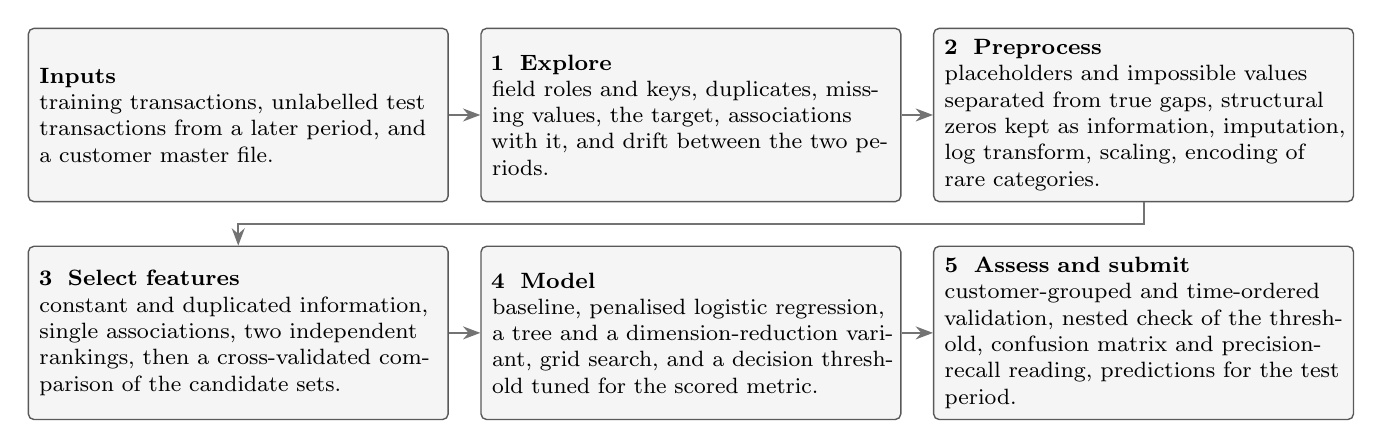
\begin{tikzpicture}[
  font=\footnotesize,
  box/.style={draw=black!65, line width=0.5pt, fill=black!4, rounded corners=2pt,
              text width=5.05cm, minimum height=2.2cm, align=left, inner sep=4pt},
  ar/.style={-{Stealth[length=2.2mm]}, draw=black!55, line width=0.7pt}]

\node[box] (a) {\textbf{Inputs}\\
  training transactions, unlabelled test transactions from a later period, and a customer master file.};

\node[box, right=0.4cm of a] (b) {\textbf{1 \ Explore}\\
  field roles and keys, duplicates, missing values, the target, associations with it, and drift between the two
  periods.};

\node[box, right=0.4cm of b] (c) {\textbf{2 \ Preprocess}\\
  placeholders and impossible values separated from true gaps, structural zeros kept as information, imputation,
  log transform, scaling, encoding of rare categories.};

\node[box, below=0.55cm of a] (d) {\textbf{3 \ Select features}\\
  constant and duplicated information, single associations, two independent rankings, then a cross-validated
  comparison of the candidate sets.};

\node[box, right=0.4cm of d] (e) {\textbf{4 \ Model}\\
  baseline, penalised logistic regression, a tree and a dimension-reduction variant, grid search, and a decision
  threshold tuned for the scored metric.};

\node[box, right=0.4cm of e] (f) {\textbf{5 \ Assess and submit}\\
  customer-grouped and time-ordered validation, nested check of the threshold, confusion matrix and
  precision-recall reading, predictions for the test period.};

\draw[ar] (a) -- (b);
\draw[ar] (b) -- (c);
\draw[ar] (c.south) -- ++(0,-0.28) -| (d.north);
\draw[ar] (d) -- (e);
\draw[ar] (e) -- (f);
\end{tikzpicture}
\end{center}

% ================================================================== 3
\section{The stages and why each one suits this data}

\lead{Preprocessing} Some amount fields held placeholders for `unknown' or impossible negative values. These
88 cells (35 placeholders, 53 negatives) became missing values, flagged rather than clipped. A further 18
negative mean purchase values (16 train, 2 test) were missed. Their totals are positive, so they look like sign
errors. They were left unchanged. Replacing them with the column median on a copy moves grouped F1 by less
than 0.001.
The 65 rows with every transaction field empty were dropped, leaving 6,469. A first or second purchase has no
history to measure: 1{,}048 training rows come from customers with zero or one earlier order, so the fields that cannot
be measured were set to zero and marked.
Amounts are skewed, so a log transform and scaling follow, and rare categories were grouped before encoding.

\lead{Integrating the customer data} The customer file is optional, and the key was checked first so no
transaction is duplicated. Region and join year differ in repeat rate, but their values are fixed per customer,
so they can work as hidden IDs. One region repeats on 94\% of its rows, yet one customer supplies 86\% of that
region's rows. Dropping all 33 customer-file columns moves grouped F1 only from 0.7484 to 0.7481, so they add
nothing measurable but do no harm. Street, company name and postal code were left out because they identify a
customer rather than describe behaviour.

\lead{Feature selection} Selection was made by concept rather than by column, because encoding one category as
several indicators makes those columns dependent. Constant and near-duplicate fields go first, then weak single
associations, then two separate rankings, and finally a cross-validated comparison of the candidate sets. The
funnel runs from 53 concepts and 124 columns to 19 and 64. The grouped folds put both within noise (0.741
against 0.748), so the model keeps all 124 columns.

\lead{Modelling} With a few thousand rows of tabular, business-readable fields, a penalised logistic regression
is the natural first choice: stable at this size, lightly tuned, and one interpretable coefficient per feature.
A decision tree and a dimension-reduction variant were fitted as checks beside an always-yes baseline; the linear
model won, 0.748 against 0.723 and 0.745 (grouped folds at 0.50, best set per model; Figure 1).

\lead{Assessment} The same customers appear many times, so a random split tests the model on rows whose customer
already helped fit it; the folds are grouped on the customer. Because the score depends on a decision threshold
as much as on the model, that threshold was tuned on out-of-fold probabilities and re-verified inside a nested
loop. A final check fits the first 80\% and scores the last 20\%.

% ================================================================== 4
\section{Results}

The grouped 0.755 (threshold tuned inside each fold; 0.748 at a fixed 0.50) is the stricter estimate, since those folds use customers the model has never met. The
time-ordered 0.795 looks higher, but the later period has more repeaters, so always-yes already scores 0.754
there. The gain over always-yes is about 0.04 in both checks. The submission scores 0.782.

\begin{center}
\begin{tabularx}{0.82\textwidth}{@{}R r r@{}}
\toprule
\textbf{Measure} & \textbf{Model F1} & \textbf{Always-yes F1}\\
\midrule
Customer-grouped CV, nested threshold & 0.755 & 0.718\\
Time-ordered check, all rows & 0.795 & 0.754\\
\quad returning customers & 0.801 & 0.762\\
\quad first appearance & 0.730 & 0.688\\
Kaggle, public part of the test set & 0.782 & --\\
\bottomrule
\end{tabularx}
\end{center}

\begin{center}
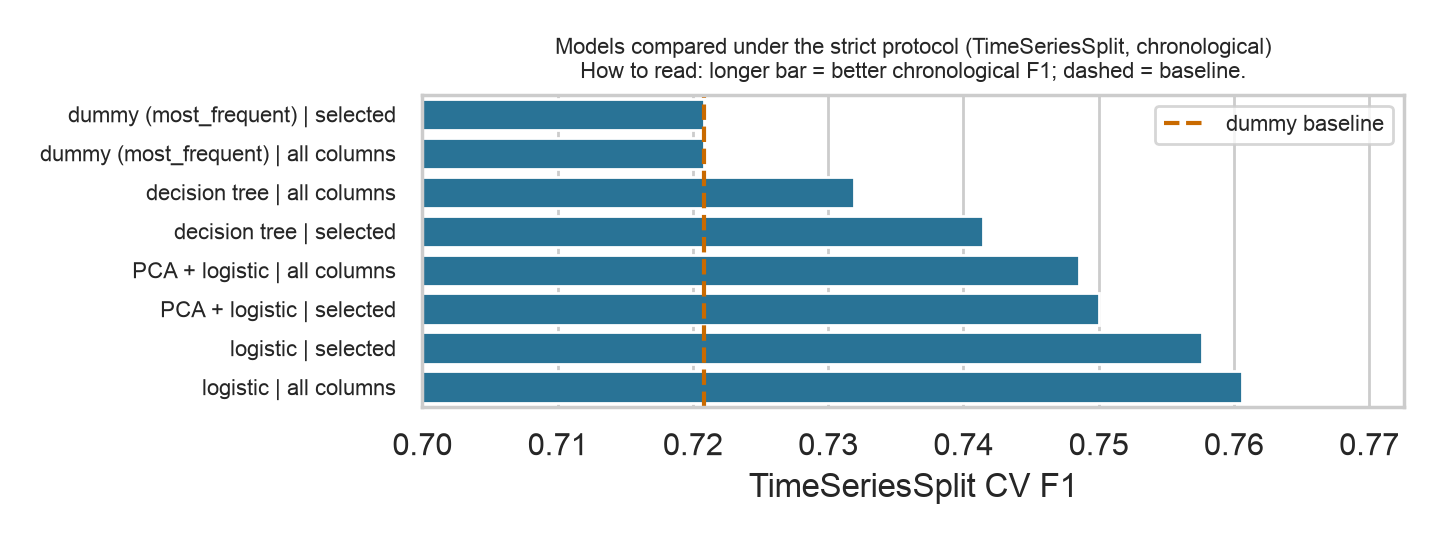
\includegraphics[width=0.55\textwidth]{figures/nb04_model_comparison.png}\\[2pt]
{\small\color{black!60} Figure 1. Every model family under the customer-grouped protocol, against the
baseline. The best model uses all 124 columns; the 64 selected columns score 0.741 (fold sd 0.0095).}\par
\vspace{2pt}
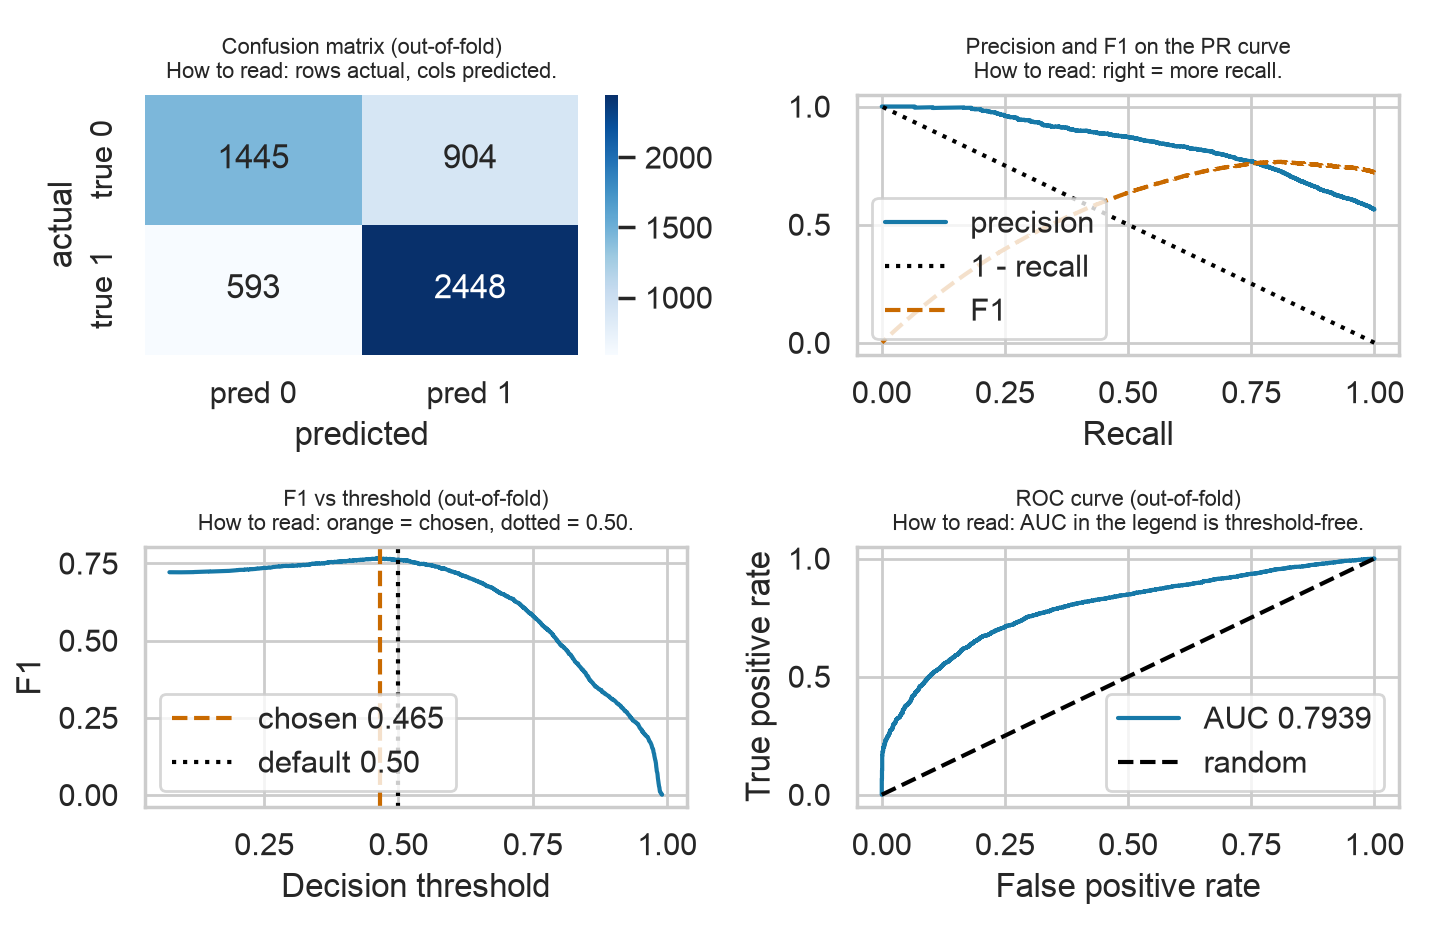
\includegraphics[width=0.55\textwidth]{figures/nb04_assessment.png}\\[2pt]
{\small\color{black!60} Figure 2. Out-of-fold results at the chosen threshold of 0.408: confusion matrix,
precision-recall trade, F1 against threshold, and ROC curve (AUC 0.792).}
\end{center}

% ================================================================== annexes
\section*{\large Annexes}
\vspace{-4pt}

\anx{A. Reproducing the work} Four notebooks, fixed seed, about two minutes. Only course-taught tools were
used: no resampling, bagging or boosting.

\anx{B. Choices that were tested and then dropped} Customer-level history features, ratios, winsorising, quartile
binning and interactions were all tried; none beat the noise between folds, and the customer aggregates made
things worse. Scaling the yes-no flags as well as the amounts was also worse.

\anx{C. Limitations} The threshold (0.408) was chosen on the training period. It flags 65.6\% of out-of-fold
predictions as repeaters against 56\% real, and 76.5\% of test rows, so it is the first value to revisit if the
private leaderboard disagrees. The transformations were fitted once on all
training rows before cross-validation; only the model is re-fitted inside each fold. The time-ordered check
reuses a subset of the training rows, so the threshold, the regularisation strength and the transformations
were all chosen with the holdout included.

\end{document}
